\documentclass{beamer}
\usepackage[utf8]{inputenc}

\usetheme{Madrid}
\usecolortheme{default}
\usepackage{amsmath,amssymb,amsfonts,amsthm}
\usepackage{txfonts}
\usepackage{tkz-euclide}
\usepackage{listings}
\usepackage{adjustbox}
\usepackage{array}
\usepackage{tabularx}
\usepackage{gvv}
\usepackage{lmodern}
\usepackage{circuitikz}
\usepackage{tikz}
\usepackage{graphicx}
\usepackage{mathtools}
\setbeamertemplate{page number in head/foot}[totalframenumber]

\usepackage{tcolorbox}
\tcbuselibrary{minted,breakable,xparse,skins}



\definecolor{bg}{gray}{0.95}
\DeclareTCBListing{mintedbox}{O{}m!O{}}{%
  breakable=true,
  listing engine=minted,
  listing only,
  minted language=#2,
  minted style=default,
  minted options={%
    linenos,
    gobble=0,
    breaklines=true,
    breakafter=,,
    fontsize=\small,
    numbersep=8pt,
    #1},
  boxsep=0pt,
  left skip=0pt,
  right skip=0pt,
  left=25pt,
  right=0pt,
  top=3pt,
  bottom=3pt,
  arc=5pt,
  leftrule=0pt,
  rightrule=0pt,
  bottomrule=2pt,
  toprule=2pt,
  colback=bg,
  colframe=orange!70,
  enhanced,
  overlay={%
    \begin{tcbclipinterior}
    \fill[orange!20!white] (frame.south west) rectangle ([xshift=20pt]frame.north west);
    \end{tcbclipinterior}},
  #3,
}
\lstset{
    language=C,
    basicstyle=\ttfamily\small,
    keywordstyle=\color{blue},
    stringstyle=\color{orange},
    commentstyle=\color{green!60!black},
    numbers=left,
    numberstyle=\tiny\color{gray},
    breaklines=true,
    showstringspaces=false,
}
%This block of code defines the information to appear in the
%Title page
\title %optional
{4.3.49}
%\subtitle{A short story}

\author % (optional)
{Vaishnavi - EE25BTECH11059}



\begin{document}


\frame{\titlepage}
\begin{frame}{Question}
Write the equation of the lines for which $\tan\theta = \frac{1}{2}$, where $\theta$ is the inclination of the line, and
\begin{enumerate}
\item[(a)] y intercept $- \frac{3}{2}$
\item[(b)] x intercept $4$
\end{enumerate}
\end{frame}
\begin{frame}{allowframebreaks}
\frametitle{Solution}
\begin{table}[H]    
  \centering
  \begin{tabular}{|c|c|}
\hline
\textbf{Name} & \textbf{Value} \\ \hline
$\vec{A}$ & $\myvec{2 & 1 \\0 & 3}$ \\ \hline
\end{tabular}

  \caption{Variables Used}
  \label{tab:1.10.2}
\end{table}

\end{frame}


\begin{frame}{Solution}
\begin{align}
\vec{A}=\myvec{
                0
                \\
                 -\frac{3}{2}  }\\
\text{Let }\vec{M}=\myvec{
                           1
                           \\
                            m
                            }\\
            \vec{M}=\myvec{
                           1
                           \\
                            \frac{1}{2}
                            }
\end{align}

\end{frame}

\begin{frame}{solution}
Let eq of line be
\begin{align}
\vec{n^T}(\vec{x}-\vec{A})=0
\end{align}
where,
\begin{align}
\vec{n^T}\vec{M}=0\\
\vec{n}=\myvec{-m
               \\
               1}\\
\vec{n}=\myvec{-\frac{1}{2}
                \\
                1}
\end{align}
\end{frame}
\begin{frame}{Solution}
Hence eq of line is
\begin{align}
\myvec{-\frac{1}{2}&1}
(\vec{x}-    
\myvec{
           0
           \\
            -\frac{3}{2}
               }   )
=0\\
\myvec{-\frac{1}{2}&1}\vec{x}
=-\frac{3}{2}
\end{align}
\end{frame}

\begin{frame}{Graph}
   Refer to Figure

\begin{figure}[H]
\begin{center}
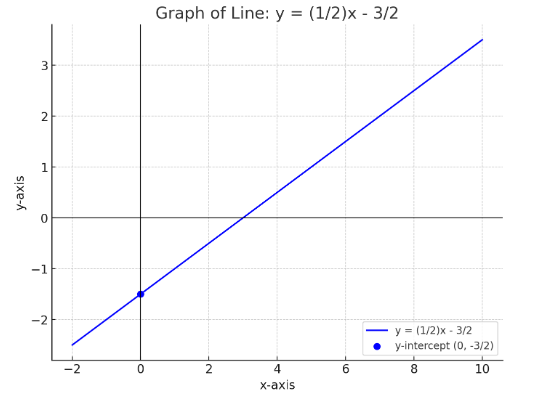
\includegraphics[width=0.6\columnwidth]{../figs/grapha.png}
\end{center}
\caption{}
\label{fig:Fig}
\end{figure}  
\end{frame}
\begin{frame}{Question}
Write the equation of the lines for which $\tan\theta = \frac{1}{2}$, where $\theta$ is the inclination of the line, and
\begin{enumerate}
\item[(a)] y intercept $- \frac{3}{2}$
\item[(b)] x intercept $4$
\end{enumerate}
\end{frame}
\begin{frame}{allowframebreaks}
\frametitle{Solution}
\begin{table}[H]    
  \centering
  \begin{table}[h!]
    \centering
    \begin{tabular}{|c|c|c|}
        \hline
        Point & For $k=3$ & For $k=-\tfrac{9}{2}$ \\
        \hline
        $A$ & $\myvec{1\\-1}$ & $\myvec{1\\-1}$ \\
$B$ & $\myvec{-4\\6}$ & $\myvec{-4\\-9}$ \\
$C$ & $\myvec{-3\\-5}$ & $\myvec{\tfrac{9}{2}\\-5}$ \\
        \hline
    \end{tabular}
    \caption{Vertices of $\triangle ABC$ after substituting $k$ values}
    \label{tab:triangle_values}
\end{table}

  \caption{Variables Used}
  \label{tab:1.10.25}
\end{table}

\end{frame}


\begin{frame}{Solution}
\begin{align}
\vec{A}=\myvec{
                4
                \\
                 0  }\\
\text{Let }\vec{M}=\myvec{
                           1
                           \\
                            m
                            }\\
            \vec{M}=\myvec{
                           1
                           \\
                            \frac{1}{2}
                            }
\end{align}

\end{frame}

\begin{frame}{solution}
Let eq of line be
\begin{align}
\vec{n^T}(\vec{x}-\vec{A})=0
\end{align}
where,
\begin{align}
\vec{n^T}\vec{M}=0\\
\vec{n}=\myvec{-m
               \\
               1}\\
\vec{n}=\myvec{-\frac{1}{2}
                \\
                1}
\end{align}

\end{frame}
\begin{frame}{Solution}
Hence eq of line is
\begin{align}
\myvec{-\frac{1}{2}&1}
(\vec{x}-    
\myvec{
           4
           \\
            0
               }   )
=0\\
\myvec{-\frac{1}{2}&1}\vec{x}
=-2
\end{align}
\end{frame}
\begin{frame}{Graph}
   Refer to Figure

\begin{figure}[H]
\begin{center}
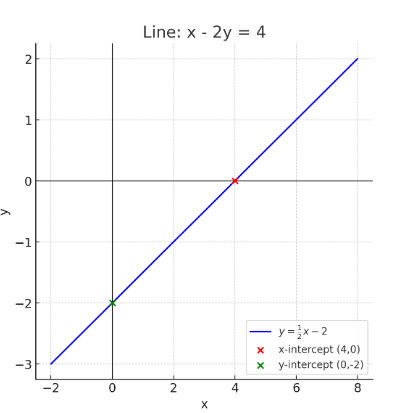
\includegraphics[width=0.6\columnwidth]{../figs/graphb.png}
\end{center}
\caption{}
\label{fig:Fig}
\end{figure}  
\end{frame}



\begin{frame}[fragile]
    \frametitle{Python Code 1}
    \begin{lstlisting}
import matplotlib.pyplot as plt
import numpy as np

# Define slope and intercept
m = 1/2
c = -3/2

# Create x values
x = np.linspace(-2, 10, 400)

# Equation of the line
y = m * x + c

# Plot the line
plt.figure(figsize=(8,6))
plt.plot(x, y, label="y = (1/2)x - 3/2", color="blue")

# Mark the y-intercept point
plt.scatter(0, c, color="blue", marker="o", label="y-intercept (0, -3/2)")

\end{lstlisting}
\end{frame}

\begin{frame}[fragile]
    \frametitle{Python Code 1}

    \begin{lstlisting}
# Draw x and y axes
plt.axhline(0, color='black', linewidth=0.8)
plt.axvline(0, color='black', linewidth=0.8)

# Labels and title
plt.xlabel("x-axis")
plt.ylabel("y-axis")
plt.title("Graph of Line: y = (1/2)x - 3/2")
plt.legend()
plt.grid(True)

# Save the graph as PNG
plt.savefig("grapha", dpi=300)

# Show plot
plt.show()


    \end{lstlisting}
\end{frame}

\begin{frame}[fragile]
    \frametitle{Python Code 2}

    \begin{lstlisting}
import matplotlib.pyplot as plt
import numpy as np

# Define the line: y = (1/2)x - 2
x = np.linspace(-2, 8, 200)
y = 0.5 * x - 2

# Create plot
plt.figure(figsize=(6,6))
plt.plot(x, y, label=r"$y=\frac{1}{2}x-2$", color="blue")

# Mark intercepts
plt.scatter([4], [0], color="red", label="x-intercept (4,0)", zorder=5)
plt.scatter([0], [-2], color="green", label="y-intercept (0,-2)", zorder=5)

# Axes
plt.axhline(0, color='black', linewidth=0.8)
plt.axvline(0, color='black', linewidth=0.8)


  \end{lstlisting}
\end{frame}
\begin{frame}[fragile]
    \frametitle{Python Code 2}

    \begin{lstlisting}
# Labels
plt.xlabel("x")
plt.ylabel("y")
plt.title("Line: x - 2y = 4")
plt.legend()
plt.grid(True)

# Save and show
file_path = "line_plot.png"   # will save in current directory
plt.savefig(file_path)
plt.show()

print(f"Plot saved as {file_path}")


  \end{lstlisting}
\end{frame}
\begin{frame}[fragile]
\frametitle{C Code}
\begin{lstlisting}
#include <stdio.h>

// Print 2x3 matrix
void printMatrix(float mat[2][3]) {
    for(int i=0; i<2; i++) {
        for(int j=0; j<3; j++) {
            printf("%6.2f ", mat[i][j]);
        }
        printf("\n");
    }
    printf("\n");
}

// Gaussian Elimination
void gaussElimination(float mat[2][3]) {
    // Normalize first row
    float factor = mat[0][0];
    if (factor != 0) {
        for(int j=0; j<3; j++)
            mat[0][j] /= factor;
    }

    \end{lstlisting}

\end{frame}

\begin{frame}[fragile]
\frametitle{C Code}
\begin{lstlisting}
   // Eliminate below
    factor = mat[1][0];
    for(int j=0; j<3; j++)
        mat[1][j] -= factor * mat[0][j];

    // Normalize second row
    factor = mat[1][1];
    if (factor != 0) {
        for(int j=0; j<3; j++)
            mat[1][j] /= factor;
    }

    // Eliminate above
    factor = mat[0][1];
    for(int j=0; j<3; j++)
        mat[0][j] -= factor * mat[1][j];
}

\end{lstlisting}
\end{frame}

\begin{frame}[fragile]
\frametitle{Python and C Code}

\begin{lstlisting}
import ctypes
import numpy as np

# Load the shared object
lib = ctypes.CDLL("./line_solver.so")

# Define function signatures
lib.gaussElimination.argtypes = [((ctypes.c_float * 3) * 2)]
lib.printMatrix.argtypes = [((ctypes.c_float * 3) * 2)]

def to_c_matrix(py_mat):
    """Convert Python 2x3 list into C float[2][3]"""
    c_mat = ((ctypes.c_float * 3) * 2)()
    for i in range(2):
        for j in range(3):
            c_mat[i][j] = py_mat[i][j]
    return c_mat
\end{lstlisting}

\end{frame}
\begin{frame}[fragile]
\frametitle{Python and C Code}

\begin{lstlisting}
def to_py_matrix(c_mat):
    """Convert C float[2][3] back to Python list"""
    return [[c_mat[i][j] for j in range(3)] for i in range(2)]

# Case (a): slope=1/2, y-intercept=-3/2
mat1 = [[0, 1, -1.5],
        [1, -0.5, 0]]

c_mat1 = to_c_matrix(mat1)
print("Case (a): before elimination:")
lib.printMatrix(c_mat1)

lib.gaussElimination(c_mat1)

\end{lstlisting}

\end{frame}
\begin{frame}[fragile]
\frametitle{Python and C Code}

\begin{lstlisting}
print("Case (a): after elimination:")
lib.printMatrix(c_mat1)
print("Python Matrix:", to_py_matrix(c_mat1))

# Case (b): slope=1/2, x-intercept=4
mat2 = [[4, 1, 0],
        [1, -0.5, 0]]

c_mat2 = to_c_matrix(mat2)
print("\nCase (b): before elimination:")
lib.printMatrix(c_mat2)

lib.gaussElimination(c_mat2)

print("Case (b): after elimination:")
lib.printMatrix(c_mat2)
print("Python Matrix:", to_py_matrix(c_mat2))


\end{lstlisting}

\end{frame}
 





\end{document}